\documentclass[12pt, AutoFakeBold]{article}

\usepackage{geometry} % 页面设置
\usepackage[hidelinks, bookmarks = true]{hyperref} % 链接
\usepackage[numbered]{bookmark} % 书签
\usepackage{xeCJK} % 中文字体
\usepackage{ctex} % 中文字体
\usepackage{titlesec} % 设置章节标题
\usepackage{anyfontsize} % 调整字号
\usepackage{indentfirst} % 首行缩进
\usepackage{titletoc} % 自定义目录
\usepackage{graphicx} % 插入图片
\usepackage{amsmath} % 数学公式
\usepackage{amssymb} % 数学符号公式
\usepackage[utf8]{inputenc} % 自定义页码
\usepackage{babel} % 自定义页码
\usepackage{float} % 浮动位置
\usepackage{xurl} % 长 url
\usepackage{caption} % 图表标注设置
\usepackage{chngcntr} % 图表记数
\usepackage{booktabs} % 表格样式
\usepackage{threeparttable} % 表格样式

\geometry{a4paper, left=3cm, right=2.5cm, top=2.5cm, bottom=2.5cm} % 页面设置
\setCJKmainfont{SimSun} % 全文宋体
\setmainfont{Source Serif Pro} % 衬线
\linespread{1.3} % 行间距最小值 20 磅
\setlength{\parindent}{2em} % 首行缩进 2 字符

\captionsetup[figure]{font={small}} % 图片标识样式设置
\counterwithin*{figure}{section} % 图片记数器
\renewcommand{\thefigure}{\thesection.\arabic{figure}} % 图片序号

\captionsetup[table]{font={small}, singlelinecheck=false, justification=raggedright} % 表格标识样式设置
\counterwithin*{table}{section} % 表格记数器
\renewcommand{\thetable}{\thesection.\arabic{table}} % 表格序号

\pagenumbering{roman} % 罗马字母标注页码
\renewcommand{\refname}{参考文献} % 重命名参考文献

\titleformat{\section}{\fontsize{16}{19}\bfseries}{\thesection}{1em}{} % 一级标题样式
% 一级标题间换页:\newpage
\titlespacing{\section}{0pt}{18pt}{12pt} % 一级标题段前段后间距

\titleformat{\subsection}{\fontsize{15}{18}\bfseries}{\thesubsection}{1em}{} % 二级标题样式
\titlespacing{\subsection}{0pt}{12pt}{6pt} % 二级标题段前段后间距

\titleformat{\subsubsection}{\fontsize{14}{17}\bfseries}{\thesubsubsection}{1em}{} % 三级标题样式
\titlespacing{\subsubsection}{0pt}{6pt}{6pt} % 三级标题段前段后间距

\renewcommand{\contentsname}{\begin{center}
\fontsize{16}{19}\bfseries 目\phantom{空格}录
\end{center}} % 重命名目录
% 自定义目录样式:一级标题
\titlecontents{section}[2.3em]
{}
{\bfseries\contentslabel[\thecontentslabel]{1.5em}}
{\hspace*{-2.3em}\bfseries}
{\titlerule*[1pc]{.}\contentspage}
% 自定义目录样式:二级标题
\titlecontents{subsection}[4.6em]
{}
{\contentslabel{2em}}
{\hspace*{-2.3em}\bfseries}
{\titlerule*[1pc]{.}\contentspage}
% 自定义目录样式:三级标题
\titlecontents{subsubsection}[6.9em]
{}
{\contentslabel{2.5em}\itshape\space}
{\hspace*{-2.3em}\bfseries}
{\titlerule*[1pc]{.}\contentspage}


% 自定义快捷命令
\newcommand{\pa}{\par ~\\} % 分段并空行
\newcommand{\R}{\mathbb{R}} % Real number domain R
\newcommand{\pr}[1]{\left(#1\right)} % ()
\newcommand{\br}[1]{\left[#1\right]} % []
\newcommand{\vr}[1]{\left\vert#1\right\vert} % ||
\newcommand{\Vr}[1]{\left\Vert#1\right\Vert} % || ||
\newcommand{\eq}[2]{\begin{equation} \label{eq:#1} #2 \end{equation}} % eq with index
\newcommand{\al}[1]{\begin{align*} #1 \end{align*}} % eq without index
\makeatletter % \fr{1, 2} for \frac{}{}
\newcommand*{\fr}[1]{%
	\fr@aux#1,,\@nil
}
\def\fr@aux#1,#2,#3\@nil{%
	\ensuremath{\frac{#1}{#2}}%
}
\makeatother


% 文档
\begin{document}
% 封面
\thispagestyle{empty}
\phantom{文件头}
\vspace{20pt}
\begin{center}

\includegraphics[width=7.5cm]{logo-1.jpg}
\end{center}
\begin{center}
{\fontsize{39}{43}\heiti 本科毕业论文}
\end{center}
\begin{center}

\includegraphics[width=4cm]{logo-2.jpg}
\end{center}
\vspace{80pt}
\begin{center}
\begin{minipage}{12.5cm}
{\fontsize{15}{18}\heiti 论文题目:} \par
\vspace{15pt}
\noindent{\fontsize{15}{18}\heiti 姓\phantom{空格}名:\hspace{8em}学\phantom{空格}号:}\par 
\vspace{15pt}
\noindent{\fontsize{15}{18}\heiti 院\phantom{空格}系:} \par
\vspace{15pt}
\noindent{\fontsize{15}{18}\heiti 专\phantom{空格}业:} \par
\vspace{15pt}
\noindent{\fontsize{15}{18}\heiti 指导老师:\hspace{8em}职\phantom{空格}称:}\par 
\vspace{15pt}
\noindent{\fontsize{15}{18}\heiti 单\phantom{空格}位:} \par
\vspace{15pt}
\noindent{\fontsize{15}{18}\heiti 完成日期:\hspace{6em} $\mathsf{2022}$\hspace{0.5em}年\hspace{0.5em}$\mathsf{0}$\hspace{0.5em}月\hspace{0.5em}$\mathsf{00}$\hspace{0.5em}日} \par
\end{minipage}
\end{center}

% 目录
\newpage
\setcounter{page}{1}
\tableofcontents	

% 中文摘要
\newpage
\section*{
\begin{center}
		摘\phantom{空格}要
\end{center}
}
\label{section:abstract-cn}
\addcontentsline{toc}{section}{摘\phantom{空格}要}
中文摘要 \pa 
\noindent \textbf{关键词:}

% 英文摘要
\newpage
\section*{
\begin{center}
		Abstract
\end{center}
}
\label{section:abstract-en}
\addcontentsline{toc}{section}{Abstract}
English abstract \pa 
\noindent \textbf{Keywords:}

% 正文
\newpage
\pagenumbering{arabic} % 改回正常页码
登革热是由登革病毒引起的一种急性虫媒传染病,主要分布于热带和亚热带地区。近几十年来,登革热蔓延到了越来越多的国家,感染登革热的人数在不断上升。至今,登革热威胁着约占全世界三分之一人口的健康,成为热带地区的一大公共卫生挑战。
\section{登革热的流行特征}
根据已有的文献研究,本部分将从传染源、传播途径、易感人群三个方面论述登革热的流行特征。
\subsection{传染源}
登革热患者、隐性感染者、带病毒的非人灵长类动物是登革热的主要传染源\cite{wang2018}。根据病毒的包膜蛋白抗原,登革病毒可分为4种血清型(DENV-1、DENV-2、DENV-3、DENV-4)。登革热的潜伏期通常为4-7天,典型症状包括高烧、头痛、呕吐、肌肉痛、关节痛和皮疹,临床诊断上容易与热带地区的其他常见传染病(如:基孔肯雅热)混淆\cite{Brady2020}。
\subsubsection{传播途径}
登革病毒主要由黑斑蚊叮咬吸血传播,在我国,白纹伊蚊和埃及伊蚊是主要传播媒介\cite{wang2018}。登革病毒也可以通过被感染的血制品及器官捐赠来传播,在新加坡等登革热流行国,估计每10000次输血中有1.6到6次可能感染登革病毒\cite{Stramer2009}。

\newpage % 一级标题分页
\section{实用样式}
以下是图 \ref{fig:map}。
\begin{figure}[H]
\centering
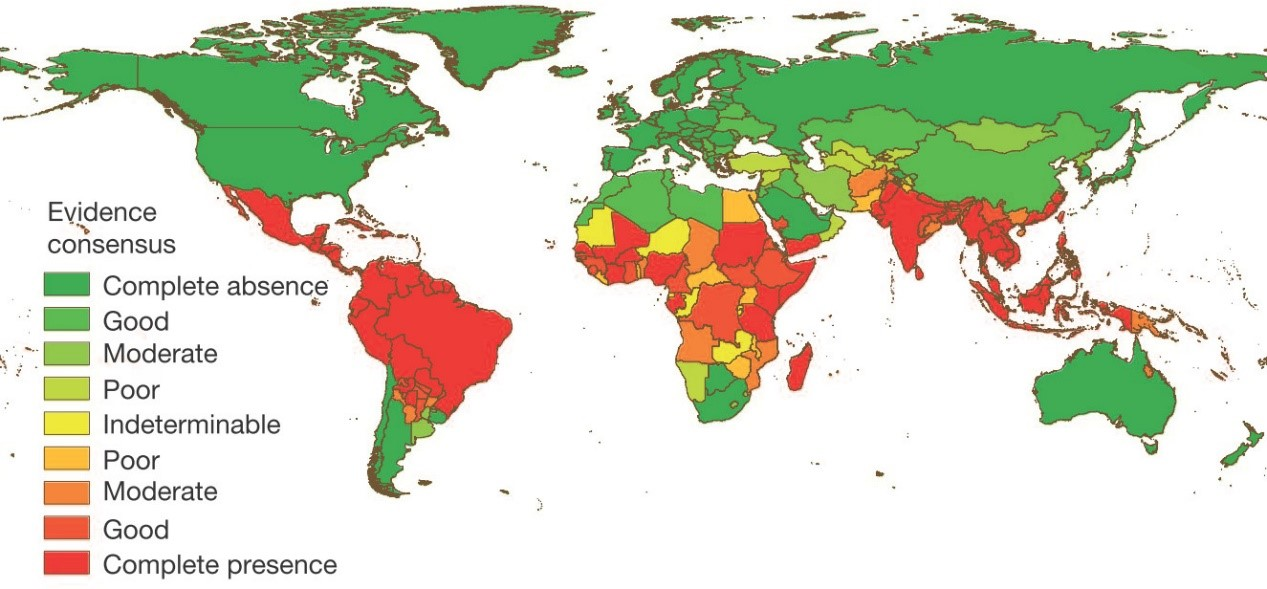
\includegraphics[width=14cm]{sample-1.jpg}
\caption{登革热在各国的流行现状} % 图片描述
\label{fig:map} % 引用标签
\end{figure}
这是一个长链接:\url{https://1234567890qwertyuiopasdfghjklzxcvbnm1234567890qwertyuiopasdfghjklzxcvbnm.com}.\par 
以下是表 \ref{table:sample}。
\begin{table}[H]
\centering
\begin{threeparttable} 
\caption{示例表格} % 表格描述
\begin{tabular}{llllllllll}
\toprule
\textbf{A} & \textbf{B} & \textbf{C} & \textbf{D} & \textbf{A} & \textbf{B} & \textbf{C} & \textbf{D} & \textbf{B} & \textbf{B} \\
\midrule
1 & 2 & 3 & 4 & 5 & 6 & 7 & 8 & 9 & 0\\
1 & 2 & 3 & 4 & 5 & 6 & 7 & 8 & 9 & 0\\
1 & 2 & 3 & 4 & 5 & 6 & 7 & 8 & 9 & 0\\
\bottomrule
\end{tabular}
\label{table:sample} % 引用标签
\end{threeparttable} 
\end{table}
\noindent 数学快捷命令示例:\\
实数集:$\R$\\
括号、分式:$$\br{\fr{a, a+b}}$$ $$\pr{\fr{c, c+d}}$$
绝对值:$$\vr{\fr{1, 1234}}$$
范式:$$\Vr{\fr{1, 1234}}$$
带标号的数学公式,以式 \ref{eq:2-1} 为例:\eq{2-1}{\int^{b}_{b-\eta}\varphi(t)dt<\fr{\varepsilon, 2\Omega}}
不带标号的数学公式,如下所示:\al{
	I &= \fr{D\pr{u, v}, D\pr{u^*, v^*}} \\
	A^* &= AI
}

% 参考文献
\newpage
\label{section:bibi}
\addcontentsline{toc}{section}{参考文献}
\begin{thebibliography}{100}
\bibitem{wang2018} 王贵强, 张复春. 中国登革热临床诊断和治疗指南[J]. 中华临床感染病杂志, 2018, 11, 5: 321-328.
\bibitem{Brady2020} \uppercase{Brady O J, Hay S I.} The global expansion of dengue: how aedes aegypti mosquitoes enabled the first pandemic arbovirus[J]. Annual Review of Entomology, 2020, 65, 1: 191-208.
\bibitem{Stramer2009} \uppercase{Stramer S L, Hollinger F B, Katz L M.} Emerging infectious disease agents and their potential threat to transfusion safety[J]. Transfusion, 2009, 49, s2: 1s-29s.
\end{thebibliography}

\end{document}